\uuid{ZbmD}
\niveau{PCSI}
\module{Analyse}
\chapitre{Généralités sur les fonctions}
\sousChapitre{Equations, inéquations}
%!TeX root=../../../encours.nouveau.tex
%%% Début exercice %%%

\duree{20}
\difficulte{1}
\auteur{Antoine Crouzet}
\datecreate{01/12/2024}
\titre{Des inégalités en tout genre}
\contenu{
\texte{Résoudre les inégalités suivantes :}
\question{$(2x+1)(3x-1)>0$}
\reponse{\begin{align*}
\begin{methode}
Dans la plupart des cas, pour déterminer le signe d'une expression, on essaie de factoriser au maximum puis de faire un tableau de signe.
\end{methode}

\begin{enumerate}
	\item On dresse le tableau de signe :
\begin{center}
  \begin{tikzpicture}
   \tkzTabInit[lgt = 3.5, espcl = 2]{$x$ / 1 , $2x+1$ / 0.6, $3x-1$ / 0.6, $(2x+1)(3x-1)$ / 0.6}{$-\infty$, $-\dfrac12$, $\dfrac13$, $+\infty$}
   \tkzTabLine{, -, z, +, t , +, }
   \tkzTabLine{, -, t, -, z , +, }
\end{align*}}
\question{$\ds{\frac{4x+3}{2x+1}\geq 0}$}
\reponse{\begin{align*}
\tkzTabLine{, +, z, -, z , +, }
\end{tikzpicture}
\end{center}
			Ainsi, \[\mathcal{S} = \left]-\infty;-\frac{1}{2}\right[\cup \left]\frac{1}{3};+\infty\right[\]
	\item On dresse le tableau de signe, en oubliant pas les doubles barres en cas de non-définition.
  \begin{center}
    \begin{tikzpicture}
     \tkzTabInit[lgt = 2.5, espcl = 2]{$x$ / 1 , $4x+3$ / 0.6, $2x+1$ / 0.6, $\dfrac{4x+3}{2x+1}$ / 1}{$-\infty$, $-\dfrac34$, $-\dfrac12$, $+\infty$}
     \tkzTabLine{, -, z, +, t , +, }
\end{align*}}
\question{$\ds{\frac{1-2x}{x+1}>0}$}
\reponse{\begin{align*}
\tkzTabLine{, -, t, -, z , +, }
     \tkzTabLine{, +, z, -, d , +, }
  \end{tikzpicture}
  \end{center}
			Ainsi, \[\mathcal{S}=\left]-\infty;-\frac{3}{4}\right] \cup \left]-\frac{1}{2};+\infty\right[\]
	\item On dresse le tableau de signe.
  \begin{center}
    \begin{tikzpicture}
     \tkzTabInit[lgt = 2.5, espcl = 2]{$x$ / 1 , $1-2x$ / 0.6, $x+1$ / 0.6, $\dfrac{1-2x}{x+1}$ / 1}{$-\infty$, $-1$, $\dfrac12$, $+\infty$}
     \tkzTabLine{, +, t, +, z , -, }
\end{align*}}
\question{$5x^2-10x+4\leq 0$}
\reponse{\begin{align*}
\tkzTabLine{, -, z, +, t , +, }
     \tkzTabLine{, -, d, +, z , -, }
  \end{tikzpicture}
  \end{center}
			Ainsi, \[\mathcal{S}=\left]-1;\frac{1}{2}\right[\]
	\item Pour les trinômes du second degré, on dispose d'un théorème. Le discriminant ici vaut $\Delta=20$, donc le trinôme dispose de deux racines : $\ds{x_1=\frac{10-\sqrt{20}}{10} \qeq x_2=\frac{10+\sqrt{20}}{10}}$. Ainsi, puisque $5>0$, on dispose du tableau de signes suivant :
  \begin{center}
\end{align*}}
\question{$\ln(2x+1)\leq \ln(x+7)$}
\reponse{\begin{align*}
\begin{tikzpicture}
     \tkzTabInit[lgt = 2.5, espcl = 2]{$x$ / 0.6 , $5x^2-10x+4$ / 0.6}{$-\infty$, $x_1$, $x_2$, $+\infty$}
     \tkzTabLine{, +, z, -, z , +, }
  \end{tikzpicture}
  \end{center}
		Ainsi \[\mathcal{S}=\interff{x_1 x_2}\]
	\item L'équation n'a de sens que si $2x+1>0$ et $x+7>0$, c'est-à-dire $x>-\frac{1}{2}$ et $x>-7$. On se place donc sur $\left]-\frac{1}{2};+\infty\right[$. Par stricte croissance de la fonction logarithme :
		\[\ln(2x+1)\leq \ln(x+7) \Leftrightarrow 2x+1\leq x+7 \Leftrightarrow x\leq 6\] Ainsi, \[\mathcal{S}=\left]-\frac{1}{2};6\right]\]
\end{align*}}
\question{$2x^3+2x\leq -2x$}
\reponse{\begin{align*}
\item On a \[2x^3+2x\leq -2x \Leftrightarrow 2x^3+4x\leq 0 \Leftrightarrow 2x(x^2+2) \leq 0\]
		$x^2+2>0$ pour tout réel $x$, donc ce produit est du signe de $2x$. Ainsi
		\[\SS=\R^-\]
	\item Les fonctions sont définies sur $\R$. On a alors
		\[2^x \geq 3^{x-1} \Leftrightarrow \eu{x\ln(2)} \geq \eu{(x-1)\ln(3)}\]
		et par stricte croissance de la fonction exponentielle sur $\R$ :
		\[2^x \geq 3^{x-1} \Leftrightarrow x\ln(2)\geq (x-1)\ln(3)\]
		soit
		\[2^x \geq 3^{x-1} \Leftrightarrow x(\ln(2)-\ln(3)) \geq -\ln(3) \Leftrightarrow x \leq \frac{-\ln(3)}{\ln(2)-\ln(3)}=\frac{\ln(3)}{\ln(3)-\ln(2)} \textrm{ car } \ln(2)-\ln(3)<0\]
\end{align*}}
\question{$2^x \geq 3^{x-1}$}
\reponse{\begin{align*}
Ainsi \[\mathcal{S}=\left]-\infty;\frac{\ln(3)}{\ln(3)-\ln(2)}\right]\]
\end{enumerate}
\end{align*}}
}

%%% Fin exercice %%%
